\documentclass{beamer}
% Load csquotes for the \enquote command
\usepackage{csquotes}
\usepackage{hyperref}
% Load biblatex for bibliography management
\usepackage[backend=biber, style=authoryear]{biblatex}
\addbibresource{bibliography.bib} % Specify your BibTeX bibliography file

\mode<presentation> {
\usetheme{CambridgeUS}
\usecolortheme{seahorse}
}

\title{Macroéconomie 1}
\author{Mart\'in Valdez}
\date{IE1}

\begin{document}

\begin{frame}
\titlepage
\end{frame}

% \begin{frame}
% \frametitle{Overview}
% \tableofcontents
% \end{frame}

% ------------------------------------------------
%  Introduction
% ------------------------------------------------
\section{Modèle de Solow}
\begin{frame}
    \frametitle{Kaldor's Stylized Facts}
    \framesubtitle{Liaison entre Empirie et Théorie Économique}
    \hypertarget{kaldor_summary}{} % Label for hyperlinks
    Les faits de Kaldor peuvent être résumés comme suit :
    \begin{itemize}
        \item  Les salaires, la production par travailleur, et le capital par travailleur 
        croissent à un taux soutenu similaire, et le rendement du capital reste sensiblement constant.
        \pause
        \item Tous les autres faits sont des corollaires à ces observations.
        \pause
        \item Nous démontrons que notre modèle de référence de la croissance économique
        est potentiellement cohérent avec tous ces faits.
    \end{itemize}
\end{frame}
\section{Modèle de Solow}
%-------------------------------------------------
%  First Macro Model: Solow Growth Model
%-------------------------------------------------

\begin{frame}
    \frametitle{Modèle de Solow}
    \framesubtitle{Introduction}
    \begin{itemize}
        \item Le modèle de Solow, développé par Solow en 1956, est utilisé pour étudier la croissance économique à long terme et les variations de revenu entre les pays.\pause
        \item \textbf{Implication principale :} 
        La productivité est \textbf{cruciale} pour la croissance économique soutenue et est 
        \textbf{plus} significative que l'accumulation de facteurs.\pause
        \item \textbf{Principaux inconvénients :}
        \begin{itemize}
            \item La productivité est considérée comme exogène.
            \item La consommation est supposée constante.
            \item Le modèle simplifie excessivement en ignorant des facteurs tels que 
            le capital humain, le progrès technologique, les imperfections du marché, 
            la diversité des agents, les rôles gouvernementaux, etc.
        \end{itemize}
    \end{itemize}
\end{frame}

\begin{frame}
    \frametitle{Modèle de Solow}
    \framesubtitle{Introduction}
    \begin{itemize}
        \item Le temps s'écoule de \( t \) (le présent) vers un futur infini.
        \item Modélise un ménage représentatif et une entreprise représentative.
        \item Considère un seul bien qui représente tout ce qui est réel dans l'économie.\pause
        \item \textbf{Fonction de production :} \( Y_t = A_t F(K_t, N_t) \)
        \begin{itemize}
            \item \( K_t \) : capital, qui est produit, utilisé pour fabriquer d'autres biens, et ne se déprécie pas complètement.
            \item \( N_t \) : travail, représentant le temps passé à utiliser les machines pour produire des biens.
            \item \( Y_t \) : production, que l'on peut considérer comme des unités de nourriture.
            \item \( A_t \) : productivité (exogène), affecte l'efficacité du capital et du travail.
        \end{itemize}
        \pause
        \item 
        Conceptualisez la production comme des \enquote{fruits}, le stock de capital comme des \enquote*{arbres fruitiers} 
        et le travail comme le temps passé à cultiver les arbres.
    \end{itemize}
\end{frame}

\begin{frame}
    \frametitle{Modèle de Solow}
    \framesubtitle{Fonction de production}
    \begin{itemize}
        \item Les deux entrées sont nécessaires : \( F(0, N_t) = F(K_t, 0) = 0 \).
        \item Augmentation avec les deux entrées : \( F_K(K_t, N_t) > 0 \) et \( F_N(K_t, N_t) > 0 \).
        \item Concavité dans les deux entrées : \( F_{KK}(K_t, N_t) < 0 \) et \( F_{NN}(K_t, N_t) < 0 \).
        \item Rendements constants à l'échelle : \( F(qK_t, qN_t) = qF(K_t, N_t) \).
        \item Le capital et le travail sont payés à leurs produits marginaux :
        \begin{itemize}
            \item \( w_t = A_t F_N(K_t, N_t) \) (taux salarial)
            \item \( R_t = A_t F_K(K_t, N_t) \) (rendement du capital)
        \end{itemize}
        (pourquoi ?)\pause
        \item Fonction de production exemple : Cobb-Douglas :
        \[ F(K_t, N_t) = K_t^\alpha N_t^{1-\alpha}, \quad 0 < \alpha < 1 \]
        \item La fonction de production est-elle réaliste ? Non ! \parencite{Banerjee_2005}.
        Alors pourquoi l'utilisons-nous ?
        
    \end{itemize}
\end{frame}

\begin{frame}
    \frametitle{Modèle de Solow}
    \framesubtitle{Consommation et Investissement}
    \begin{itemize}
        \item Les fruits peuvent être consommés (consommation) ou replantés dans le sol (investissement), 
        ce qui produit ensuite un autre arbre (capital) avec un délai d'un période.
        \item On suppose qu'une fraction constante de la production, 
        \( 0 \leq s \leq 1 \), est investie. 
        Ceci est le "taux d'épargne" ou "taux d'investissement." 
        (Plus de détails plus tard !)
        \pause
        \item \textbf{Contrainte de ressources :} \( Y_t = C_t + I_t \)
        (\enquote{Fermeture du modèle})\pause
        \item Équation d'accumulation du capital avec un taux de dépréciation \( 0 < \delta < 1 \) :
        \[ K_{t+1} = I_t + (1 - \delta)K_t \]
    \end{itemize}
\end{frame}


\begin{frame}
    \frametitle{Modèle de Solow}
    \framesubtitle{Équation Centrale et Dynamique}
    \begin{itemize}
        \item Équations simplifiées :
        \begin{align*}
            Y_t &= A_t F(K_t, N_t) \\
            C_t &= (1 - s)Y_t \\
            I_t &= sY_t \\
            w_t &= A_t F_N(K_t, N_t) \\
            R_t &= A_t F_K(K_t, N_t)
        \end{align*}
        \item Combinez les quatre premières équations en une seule équation dynamique centrale
        \pause
        \[ K_{t+1} = sA_t F(K_t, N_t) + (1 - \delta)K_t \]
        \item Supposez que \( A_t = A \) et \( N_t = N \), et
        définissez les variables par travailleur : \( k_t = \frac{K_t}{N} \)
        \item Dynamique par travailleur : \( k_{t+1} = sA_t f(k_t) + (1 - \delta)k_t \)
    \end{itemize}
\end{frame}

\begin{frame}
    \frametitle{Modèle de Solow}
    \framesubtitle{L'état Stationnaire}
    \begin{itemize}
        \item Le stock de capital à l'état stationnaire, \( k^* \), est là où \( k_{t+1} = k_t \).
        \item Graphiquement, c'est là où la courbe de \( k_{t+1} \) croise la ligne à 45 degrés.
        \item Sous les hypothèses de la fonction de production et des conditions d'Inada, il existe un stock de capital à l'état stationnaire non nul.
        \item Stabilité : Pour toute valeur initiale \( k_t \neq 0 \), le stock de capital converge vers ce point.
        \item Implications : Une fois le capital atteint \( k^* \), toutes les autres variables se stabilisent également à leurs valeurs à l'état stationnaire, régies par \( k^* \).
        \item Exemple avec Cobb-Douglas : \( f(k_t) = k_t^\alpha \)
    \end{itemize}
\end{frame}

\begin{frame}
    \frametitle{Modèle de Solow}
    \framesubtitle{Analyse Graphique de l'État Stationnaire}
    \begin{figure}
        \centering
        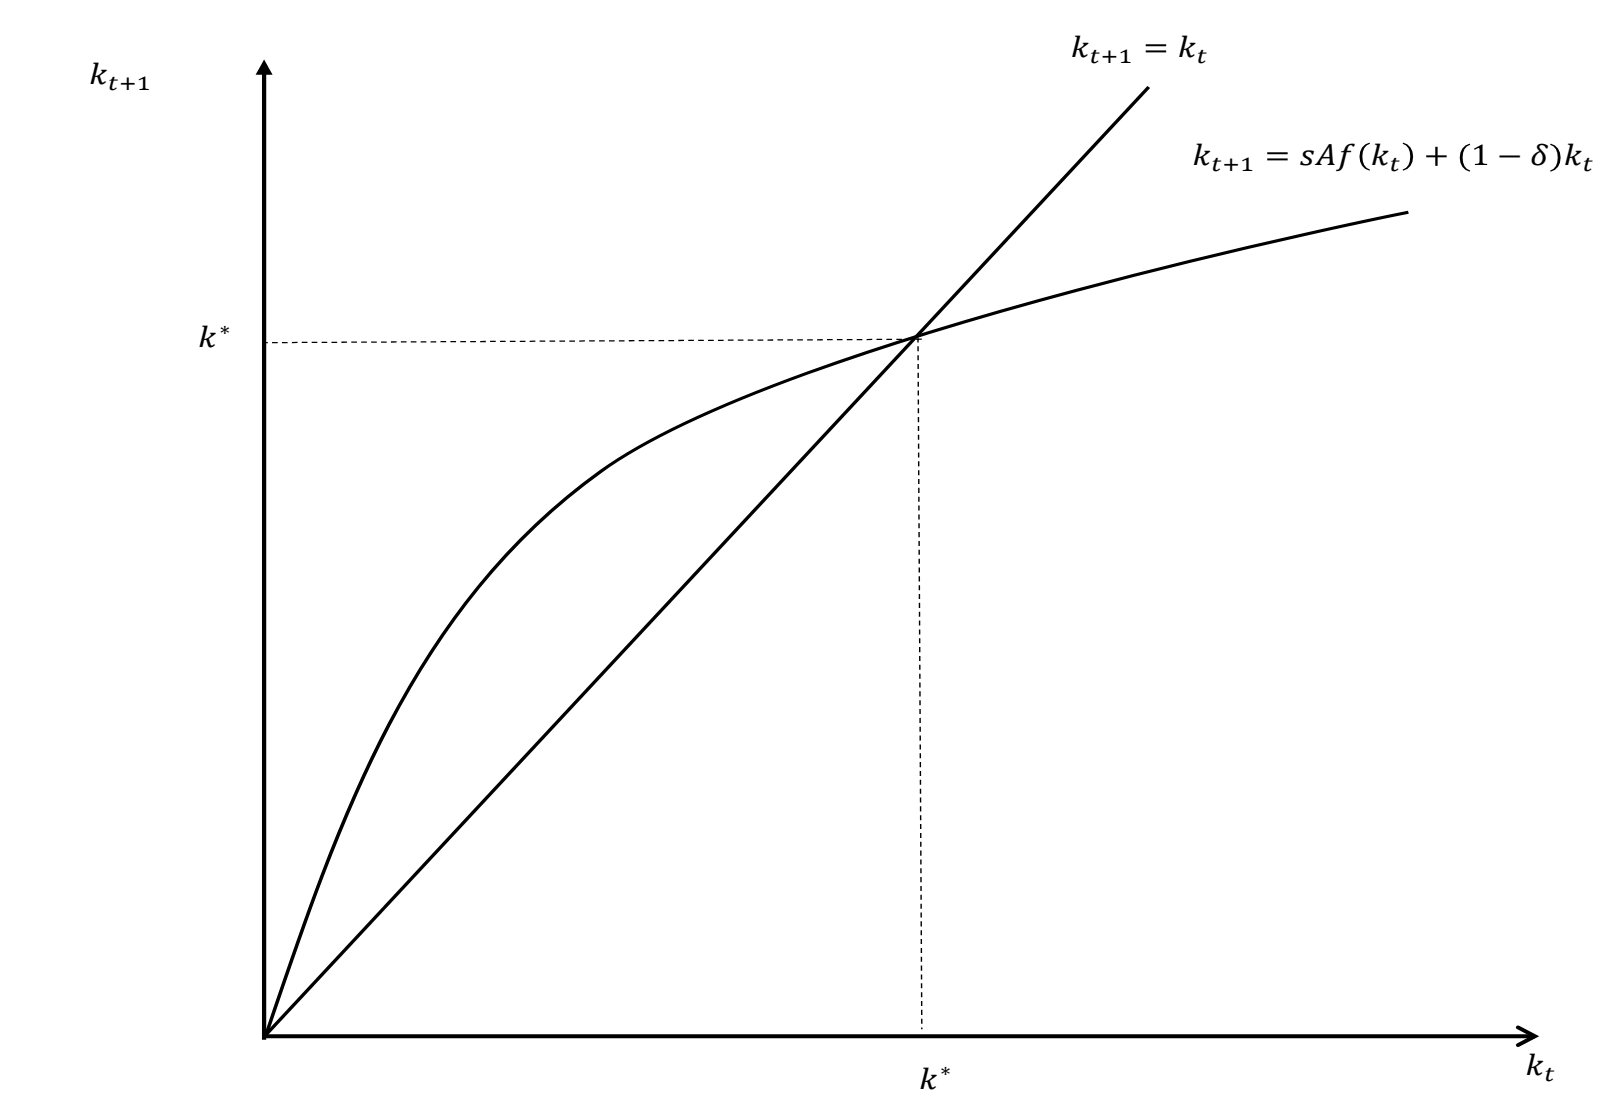
\includegraphics[width=0.65\textwidth]{graphs/ss_solow.png} % Ensure the image file is in the same directory as your .tex file or provide the relative path
        \caption{
        \footnotesize Représentation graphique de la convergence vers 
        l'état stationnaire \( k^* \) dans le modèle de Solow. 
        La courbe illustre comment le capital par travailleur \( k_t \) évolue vers 
        \( k^* \), où la courbe de \( k_{t+1} \) croise la ligne à 45 degrés.
        \textit{Source:} \textcite{Garin_etal_2021}}
    \end{figure}
\end{frame}

\begin{frame}
    \frametitle{Modèle de Solow}
    \framesubtitle{Solutions de l'État Stationnaire}
    
    \[
    k^* = \left(\frac{sA}{\delta}\right)^{\frac{1}{1-\alpha}}.
    \]

    \vspace*{5pt}

    \pause
    \vspace*{5pt}


    Les valeurs à l'état stationnaire pour d'autres variables sont:
    
    \textbf{Production par travailleur:} \( y^* = Ak^{* \alpha} \)
    
    \textbf{Consommation par travailleur:} \( c^* = (1 - s)Ak^{* \alpha} \)
    
    \textbf{Investissement par travailleur:} \( i^* = sAk^{* \alpha} \)
    
    \textbf{Rendement du capital:} \( R^* = \alpha Ak^{* \alpha - 1} \)
    
    \textbf{Salaire par travailleur:} \( w^* = (1 - \alpha) Ak^{* \alpha} \)
\end{frame}

\begin{frame}
    \frametitle{Modèle de Solow}
    \framesubtitle{Évaluation de l'Impact d'un Taux d'Épargne Plus Élevé}
    \textbf{Questions:} 
    \begin{itemize}
        \item 
        Comment un taux d'épargne plus élevé
        ou une augmentation de la productivité  (\( A \))
         influence-t-il l'accumulation de capital et 
        la croissance économique à long terme?
    \end{itemize}
\end{frame}

\begin{frame}
    \frametitle{Modèle de Solow}
    \framesubtitle{Analyse Graphique - Taux d'Épargne et Accumulation de Capital}

    \begin{figure}
        \centering
        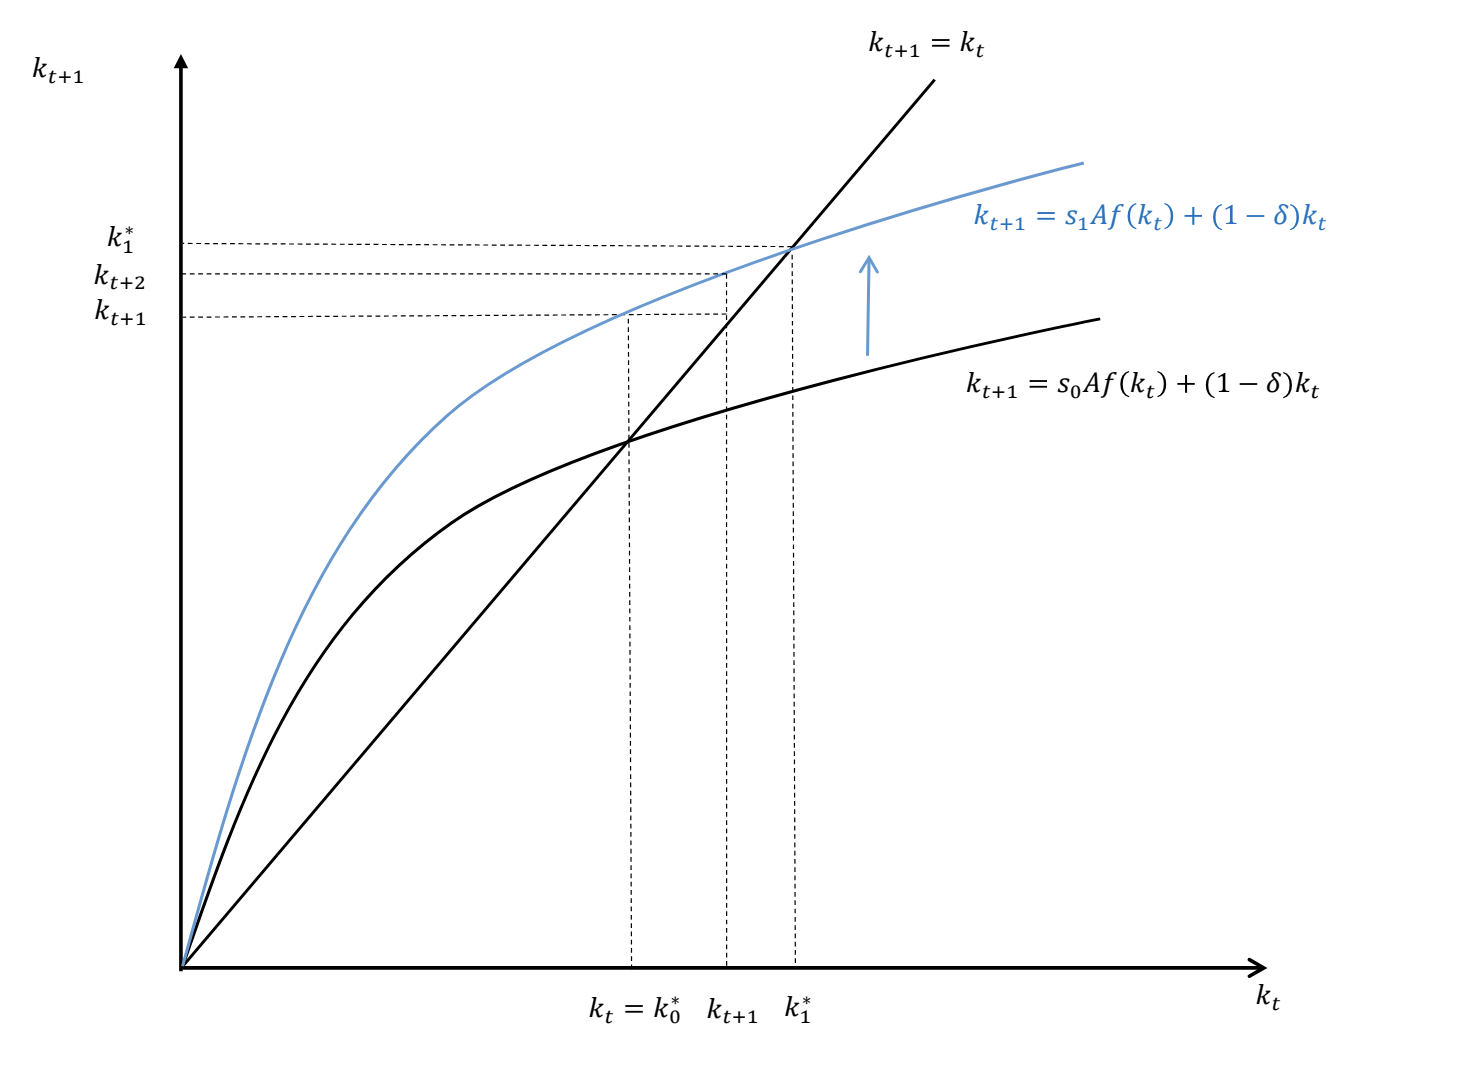
\includegraphics[width=0.65\textwidth]{graphs/ss_solow_s2.png} % Update the path to your actual image file
        \caption{
            \footnotesize \textit{Source: }\textcite{Garin_etal_2021}
        }
    \end{figure}
\end{frame}


\begin{frame}
    \frametitle{Taux d'Épargne Optimal \( s \)}
    \framesubtitle{Règle d'Or pour Maximiser \( c^* \)}

    \textbf{Quelle est la valeur optimale du taux d'épargne \( s \) ?}
    \begin{itemize}
        \item L'utilité provient de la consommation, non de la production.
        \item Un taux d'épargne plus élevé \( s \) :
            \begin{itemize}
                \item Augmente le capital \(\rightarrow\) plus de production \(\rightarrow\) plus de consommation
                \item Réduit la part consommée \(\rightarrow\) moins de consommation
            \end{itemize}
        \item \textbf{Règle d'Or :} Maximiser \( c^* = (1-s)y^* \)
            \begin{itemize}
                \item \( s = 0 \) et \( s = 1 \) : \( c^* = 0 \)
            \end{itemize}
        \item Condition : \(\frac{dc^*}{ds} = -y^* + (1-s)\frac{dy^*}{ds} = 0\)
        \item Équilibre entre réduire la part consommée et augmenter la production.
        \item Est-ce une bonne description du comportement de consommation dans le monde réel ?
    \end{itemize}
\end{frame}


%-------------------------------------------------
%  Graphs
%-------------------------------------------------


\end{document}
